\documentclass[11pt]{article}
\usepackage[margin=0.72in]{geometry}
\usepackage{graphicx}
\usepackage{booktabs}
\usepackage{amsmath}
\usepackage{amssymb}
\usepackage{float}
\usepackage{hyperref}
\usepackage{xcolor}
\usepackage{tikz}
\usetikzlibrary{arrows.meta,positioning}
\hypersetup{colorlinks=true,linkcolor=blue,urlcolor=blue}

\title{\textbf{CSIT 595 Special Topics for GenAI\\ Assignment 1 \\ \large Neeraj Kumar Singh (50161746)}\\
Generative Trilemma: VAE, GAN, and Diffusion on Fashion-MNIST}
\author{}
\date{}

\newcommand{\img}[2]{\begin{figure}[H]\centering
\includegraphics[width=0.86\textwidth]{#1}
\caption{#2}\end{figure}}
\newcommand{\code}[1]{\texttt{#1}}
\tikzset{
  archbox/.style={draw, rounded corners, align=center, minimum height=0.65cm,
    text width=2.45cm, fill=blue!6, font=\scriptsize},
  archarrow/.style={-{Latex[length=2mm]}, thick},
}

\begin{document}
\maketitle

\section*{Objective}

This assignment implements and evaluates three generative models on the same dataset:
\begin{itemize}
\item Variational Autoencoder (VAE);
\item Generative Adversarial Network (GAN); and
\item an unconditional diffusion model (DDPM-style).
\end{itemize}

The comparison is organized as a practical generative trilemma:
\begin{enumerate}
\item sample quality (realism);
\item diversity and coverage (mode coverage); and
\item sampling cost (inference speed).
\end{enumerate}

All models are unconditional. Class labels are never used as generator or denoiser inputs; they are used only to train the evaluator and analyze generated samples afterward.

\section*{Dataset}

Fashion-MNIST contains 28~$\times$~28 grayscale images from ten classes. For consistency across all models, each image is padded to 32~$\times$~32 with one channel and normalized to approximately $[-1,1]$ using
\[
x_{\mathrm{normalized}}=\frac{x-0.5}{0.5}.
\]

\section{Common Setup + Evaluator Network}

\subsection{Preprocessing}

The shared PyTorch data loader uses Fashion-MNIST, padding by two pixels on every side, converting to a tensor, and applying the normalization above. Images have shape $(N,1,32,32)$ and are loaded with batch size 128.

\subsection{Architecture and hyperparameters}

The following settings were used in the final full run. They are reported explicitly to make the comparison reproducible.

\begin{table}[H]
\centering
\scriptsize
\caption{Architecture and optimization hyperparameters.}
\begin{tabular}{p{0.17\textwidth}p{0.38\textwidth}p{0.34\textwidth}}
\toprule
\textbf{Component} & \textbf{Architecture} & \textbf{Training hyperparameters}\\
\midrule
Evaluator CNN &
Conv $(1\rightarrow32)$, Conv $(32\rightarrow64)$, Conv $(64\rightarrow128)$; batch normalization, ReLU, and $2\times2$ max pooling after the first two blocks, followed by adaptive average pooling; Linear $(128\rightarrow64\rightarrow10)$ classifier. The 64-dimensional hidden layer before the final classifier is used for cFID features. &
Adam, learning rate $1\times10^{-3}$; cross-entropy loss; 10 epochs.\\
\midrule
VAE &
Encoder channels $1\rightarrow32\rightarrow64\rightarrow128\rightarrow128$ with stride-2 convolutions; latent mean and log-variance of dimension 64; decoder starts from $128\times4\times4$ and uses transposed-convolution channels $128\rightarrow64\rightarrow32\rightarrow1$ with final $\tanh$. &
Adam, learning rate $2\times10^{-4}$; 25 epochs; mean pixel reconstruction MSE plus $0.1$ times mean per-latent-dimension KL; latent prior $\mathcal{N}(0,I)$.\\
\midrule
GAN &
Generator latent dimension 128; transposed-convolution channels $128\rightarrow256\rightarrow128\rightarrow64\rightarrow1$, batch normalization, ReLU, final $\tanh$. Discriminator convolution channels $1\rightarrow64\rightarrow128\rightarrow256\rightarrow1$, LeakyReLU slope 0.2 and batch normalization in intermediate blocks. &
Adam for both networks, learning rate $2\times10^{-4}$, betas $(0.5,0.999)$; binary cross-entropy with logits; 25 epochs.\\
\midrule
DDPM-style model &
Compact U-Net with base channels 32; down path $1\rightarrow32\rightarrow64\rightarrow128$; two-block $128$-channel middle; up path $128\rightarrow64\rightarrow32\rightarrow1$ with skip additions; GroupNorm and SiLU; sinusoidal timestep features of dimension 64. &
AdamW, learning rate $2\times10^{-4}$; 20,000 optimization steps; MSE noise-prediction loss; $T=500$ forward timesteps; linear $\beta$ schedule from $10^{-4}$ to $0.02$.\\
\bottomrule
\end{tabular}
\end{table}

All models use batch size 128, one grayscale input channel, 32~$\times$~32 images, and the same unconditional training protocol. The evaluator uses labels only for classifier training; labels are not supplied to the VAE, GAN, or diffusion model.

\begin{figure}[H]
\centering
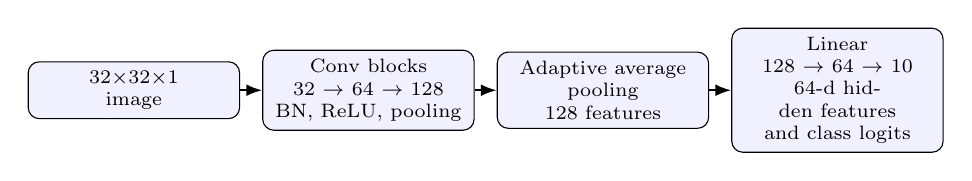
\begin{tikzpicture}[node distance=0.22cm and 0.28cm]
\node[archbox] (input) {32$\times$32$\times$1\\image};
\node[archbox, right=of input] (conv) {Conv blocks\\32 $\rightarrow$ 64 $\rightarrow$ 128\\BN, ReLU, pooling};
\node[archbox, right=of conv] (pool) {Adaptive average\\pooling\\128 features};
\node[archbox, right=of pool] (class) {Linear\\128 $\rightarrow$ 64 $\rightarrow$ 10\\64-d hidden features\\and class logits};
\draw[archarrow] (input)--(conv);
\draw[archarrow] (conv)--(pool);
\draw[archarrow] (pool)--(class);
\end{tikzpicture}
\caption{Evaluator CNN architecture. The 64-dimensional hidden layer immediately before the final classifier is used for cFID features.}
\end{figure}

\subsection{Evaluator CNN}

A small CNN is trained on Fashion-MNIST labels for ten epochs. It contains three convolutional feature blocks, adaptive average pooling, and fully connected classification layers. The final test accuracy was:
\[
\boxed{0.8292}.
\]

\img{codes/report_figures/evaluator_training_results.png}
{Evaluator CNN training loss over 10 epochs. The final held-out Fashion-MNIST test accuracy is 0.8292; the final training accuracy is 0.9240.}

\begin{table}[H]\centering
\caption{Evaluator task results.}
\begin{tabular}{ll}
\toprule
\textbf{Evaluator deliverable} & \textbf{Result}\\
\midrule
Training epochs & 10\\
Final training loss & 0.2102\\
Final training accuracy & 0.9240\\
Test accuracy & \textbf{0.8292}\\
Feature dimension & 64\\
Use of labels during generation & None\\
\bottomrule
\end{tabular}
\end{table}

The evaluator is trained only to provide a common, held-out assessment pipeline. Labels are not passed to any generator or denoiser. The final test accuracy is 0.8292, compared with a final training accuracy of 0.9240. Most errors are expected among visually similar classes (T-shirt, pullover, coat, and shirt; sneaker and ankle boot). The evaluator-based histograms, entropy, and KL values should therefore be read as approximate.

\subsection{Feature extractor and cFID}

The 64-dimensional hidden representation immediately before the evaluator final classifier is used as a feature extractor. For real and generated feature sets, a lightweight FID-like score is calculated:
\[
\mathrm{cFID}=\|\mu_r-\mu_g\|_2^2+
\operatorname{Tr}\left(\Sigma_r+\Sigma_g-
2\left(\Sigma_r^{1/2}\Sigma_g\Sigma_r^{1/2}\right)^{1/2}\right).
\]
Lower cFID indicates closer agreement with the real feature distribution. This is an evaluator-feature cFID-style metric, not standard Inception FID.

The evaluator produces the real reference feature distribution from held-out test images and produces generated feature distributions for each of the VAE, GAN, and diffusion models. Because these are 64-dimensional evaluator features, the cFID scale is not directly comparable with standard Inception FID values. The resulting cFID values are reported in the individual model sections and in the final comparison table.

\subsection{Coverage metrics}

The evaluator predicts labels for generated images. From the ten-class generated histogram, the experiment reports:
\begin{itemize}
\item the generated label histogram;
\item label entropy, where higher is better and the ten-class maximum is $\ln(10)\approx2.303$; and
\item KL divergence from the real label distribution, where lower is better.
\end{itemize}

The generated ten-class histograms, entropy, and KL divergence values are reported for each model below. Thus, the evaluator section defines the shared measurement procedure, while the model sections report the corresponding evaluator-based results.

\begin{table}[H]
\centering
\scriptsize
\caption{Evaluator-predicted coverage metrics for generated images. Histogram entries are class probabilities for evaluator classes 0 through 9.}
\begin{tabular}{lccc}
\toprule
\textbf{Model} & \textbf{Generated label histogram (classes 0--9)} & \textbf{Entropy} & \textbf{KL divergence}\\
\midrule
VAE &
\begin{tabular}{c}
[0.0370, 0.1335, 0.1105, 0.2465, 0.0135,\\
0.0215, 0.0545, 0.0060, 0.1045, 0.2725]
\end{tabular}
& 1.900 & 0.426\\
GAN &
\begin{tabular}{c}
[0.0565, 0.1850, 0.0575, 0.1455, 0.0675,\\
0.1405, 0.0825, 0.0465, 0.0925, 0.1260]
\end{tabular}
& \textbf{2.207} & \textbf{0.106}\\
DDPM &
\begin{tabular}{c}
[0.0230, 0.1100, 0.0585, 0.1370, 0.0610,\\
0.0955, 0.0790, 0.0035, 0.2155, 0.2170]
\end{tabular}
& 2.045 & 0.277\\
\bottomrule
\end{tabular}
\end{table}

The histograms are normalized to sum to one. Entropy is computed from each generated histogram, and KL divergence is computed from the generated distribution relative to the real Fashion-MNIST label distribution. The GAN has the most balanced histogram, although its class 1 share is still 18.5\%. The VAE is concentrated in classes 9, 3, and 1, while the DDPM histogram is concentrated mainly in classes 8 and 9.

\subsection{Sampling cost}

Sampling speed is measured in images per second with CUDA synchronization before and after generation. The reported time for 5,000 images is estimated from the measured throughput:
\[
t_{5000}=t_{\mathrm{measured}}\frac{5000}{N_{\mathrm{measured}}}.
\]

Sampling cost is measured after generation by each model's sampler, with the evaluator used afterward only for labels and features. The measured images/sec and estimated time for 5,000 images are reported in the VAE, GAN, diffusion, and final comparison tables.

\section{Variational Autoencoder (VAE)}

\subsection{Implementation and objective}

The VAE is an unconditional convolutional encoder-decoder. The encoder predicts a latent mean and log-variance; the reparameterization trick produces a latent sample; and the decoder reconstructs a 32~$\times$~32 image. Training minimizes reconstruction loss plus KL divergence:
\[
\mathcal{L}_{\mathrm{VAE}}=
\mathcal{L}_{\mathrm{reconstruction}}+
\beta D_{\mathrm{KL}}(q(z|x)\|p(z)).
\]
The latent dimension is 64. The reconstruction term is the mean pixel MSE, while the KL term is averaged over both the batch and the 64 latent dimensions; thus the implemented objective is mean pixel MSE plus $0.1$ times mean per-latent-dimension KL. The optimizer is Adam with learning rate $2\times10^{-4}$. The VAE was trained for 25 epochs. The full VAE contains 790,081 parameters; prior sampling uses only its decoder and latent projection, which contain 297,569 parameters.

\begin{figure}[H]
\centering
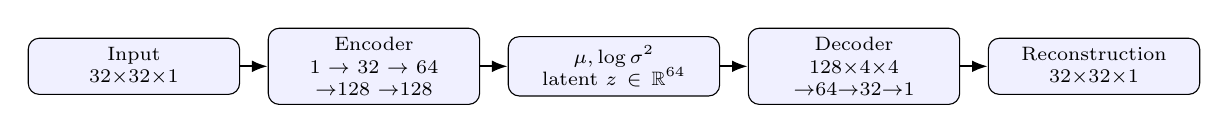
\begin{tikzpicture}[node distance=0.22cm and 0.35cm]
\node[archbox] (x) {Input\\32$\times$32$\times$1};
\node[archbox, right=of x] (enc) {Encoder\\1 $\rightarrow$ 32 $\rightarrow$ 64\\$\rightarrow$128 $\rightarrow$128};
\node[archbox, right=of enc] (latent) {$\mu,\log\sigma^2$\\latent $z\in\mathbb{R}^{64}$};
\node[archbox, right=of latent] (dec) {Decoder\\128$\times$4$\times$4\\$\rightarrow$64$\rightarrow$32$\rightarrow$1};
\node[archbox, right=of dec] (out) {Reconstruction\\32$\times$32$\times$1};
\draw[archarrow] (x)--(enc);
\draw[archarrow] (enc)--(latent);
\draw[archarrow] (latent)--(dec);
\draw[archarrow] (dec)--(out);
\end{tikzpicture}
\caption{VAE architecture. The latent vector is sampled using the reparameterization trick.}
\end{figure}

\subsection{Training curves}

\img{codes/report_figures/vae_losses.png}
{VAE training curves over 25 epochs: reconstruction loss (blue), KL divergence term (orange), and total loss (green). Reconstruction and total losses decrease steadily throughout training. The KL term falls to its minimum (about 0.213) around epoch 7 and then rises slightly to 0.226, as the encoder uses more of the latent space to improve reconstructions.}

\subsection{Required visualizations}

\img{codes/assignment1_outputs/vae_reconstruction.png}
{VAE reconstruction grid: original images and their reconstructions.}

\img{codes/assignment1_outputs/vae_samples.png}
{VAE unconditional samples from the prior $z\sim\mathcal{N}(0,I)$. 100 samples shown as a $10\times10$ grid.}

\img{codes/assignment1_outputs/vae_interpolation.png}
{VAE latent interpolation between two real test images (an ankle boot and a pullover). Both images are encoded to their latent means, and 10 evenly spaced points on the line between them are decoded.}

\subsection{Evaluation}

The VAE results were:
\[
\mathrm{cFID}=32.808,\qquad
\mathrm{entropy}=1.900,\qquad
\mathrm{KL}=0.426,
\]
with 59,841.06 images/sec and an estimated 0.084 seconds for 5,000 images. The VAE is fast and stable, but its images are smoother and blurrier than the GAN samples.

\section{GAN}

\subsection{Implementation}

The GAN is an unconditional DCGAN-style generator and discriminator. The generator maps random latent vectors to 32~$\times$~32 images and the discriminator distinguishes real training images from generated images. The GAN was trained for 25 epochs.

The generator uses a 128-dimensional Gaussian noise vector. Both generator and discriminator use Adam with learning rate $2\times10^{-4}$ and betas $(0.5,0.999)$. Training uses binary cross-entropy with logits. The generator uses transposed-convolution channels $128\rightarrow256\rightarrow128\rightarrow64\rightarrow1$; the discriminator uses convolution channels $1\rightarrow64\rightarrow128\rightarrow256\rightarrow1$.

\begin{figure}[H]
\centering
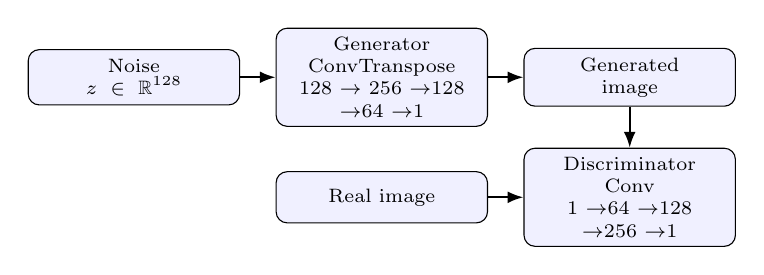
\begin{tikzpicture}[node distance=0.24cm and 0.45cm]
\node[archbox] (z) {Noise\\$z\in\mathbb{R}^{128}$};
\node[archbox, right=of z] (gen) {Generator\\ConvTranspose\\128 $\rightarrow$ 256 $\rightarrow$128\\$\rightarrow$64 $\rightarrow$1};
\node[archbox, right=of gen] (fake) {Generated\\image};
\node[archbox, below=0.52cm of fake] (disc) {Discriminator\\Conv\\1 $\rightarrow$64 $\rightarrow$128\\$\rightarrow$256 $\rightarrow$1};
\node[archbox, left=of disc] (real) {Real image};
\draw[archarrow] (z)--(gen);
\draw[archarrow] (gen)--(fake);
\draw[archarrow] (fake)--(disc);
\draw[archarrow] (real)--(disc);
\end{tikzpicture}
\caption{GAN architecture. The discriminator receives real and generated images and provides the adversarial signal.}
\end{figure}

\subsection{Training curves}

\img{codes/report_figures/gan_losses.png}
{GAN training curves over 25 epochs: generator loss (blue) and discriminator loss (orange). After epoch 4 the generator loss rises steadily (1.60 to 2.56) while the discriminator loss falls (0.84 to 0.47), indicating that the discriminator gradually gains the upper hand; training does not diverge.}

\subsection{Required visualizations}

\img{codes/assignment1_outputs/gan_samples.png}
{GAN unconditional samples. 100 samples shown as a $10\times10$ grid.}

\img{codes/assignment1_outputs/gan_interpolation.png}
{GAN latent interpolation: 10 evenly spaced points between two random latent vectors $z_0, z_1 \sim \mathcal{N}(0,I)$, decoded by the generator.}

\img{codes/assignment1_outputs/gan_mode_collapse_checkpoints.png}
{Mode-collapse watch: evaluator-predicted label histograms of 2,000 generated samples after every GAN epoch. At epoch 1 the generator is partially collapsed: 31.5\% of samples are classified as class 1 (trouser), while classes 0, 2, and 7 receive 0.35\%, 0.05\%, and 0\%, respectively. Coverage improves over training, and class 1 falls to 17.7\% at the epoch-25 checkpoint and 18.5\% in the final evaluation.}

\subsection{Evaluation}

The GAN results were:
\[
\mathrm{cFID}=0.978,\qquad
\mathrm{entropy}=2.207,\qquad
\mathrm{KL}=0.106,
\]
with 14,082.14 images/sec and an estimated 0.355 seconds for 5,000 images. Its generated histogram was
\[
[0.0565,0.1850,0.0575,0.1455,0.0675,
0.1405,0.0825,0.0465,0.0925,0.1260].
\]
The GAN histogram is the most balanced of the three models and its entropy is the highest, although class 1 (trouser) remains over-represented at 18.5\%. The GAN produced the best measured quality and coverage in this rerun.

\section{Diffusion Model}

\subsection{Forward process}

The diffusion model uses a linear noise schedule with $T=500$ forward timesteps:
\[
x_t=\sqrt{\bar{\alpha}_t}x_0+
\sqrt{1-\bar{\alpha}_t}\epsilon,\qquad
\epsilon\sim\mathcal{N}(0,I).
\]

The denoiser is a compact U-Net with 32 base channels and 64-dimensional sinusoidal timestep embeddings. Its down path increases channels from 32 to 64 to 128, the middle contains two 128-channel convolutional blocks, and the up path returns to one output channel through skip additions. GroupNorm and SiLU activations are used in the down, middle, and up blocks. The linear beta schedule ranges from $10^{-4}$ to $0.02$.

\begin{figure}[H]
\centering
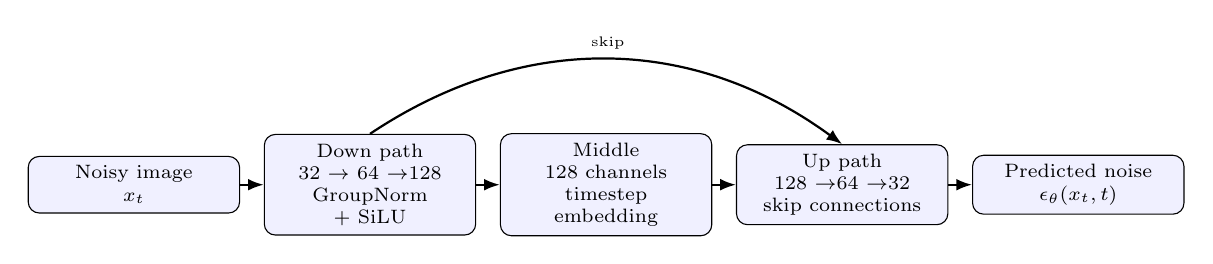
\begin{tikzpicture}[node distance=0.22cm and 0.3cm]
\node[archbox] (noisy) {Noisy image\\$x_t$};
\node[archbox, right=of noisy] (down) {Down path\\32 $\rightarrow$ 64 $\rightarrow$128\\GroupNorm + SiLU};
\node[archbox, right=of down] (mid) {Middle\\128 channels\\timestep embedding};
\node[archbox, right=of mid] (up) {Up path\\128 $\rightarrow$64 $\rightarrow$32\\skip connections};
\node[archbox, right=of up] (pred) {Predicted noise\\$\epsilon_\theta(x_t,t)$};
\draw[archarrow] (noisy)--(down);
\draw[archarrow] (down)--(mid);
\draw[archarrow] (mid)--(up);
\draw[archarrow] (up)--(pred);
\draw[archarrow] (down.north) to[bend left=35] node[above,font=\tiny]{skip} (up.north);
\end{tikzpicture}
\caption{DDPM-style denoiser architecture. A sinusoidal timestep embedding conditions the compact U-Net.}
\end{figure}

\subsection{Training}

At each optimization step, a random timestep $t$ and Gaussian noise $\epsilon$ are sampled. A compact U-Net predicts $\epsilon_\theta(x_t,t)$, and training minimizes:
\[
\mathcal{L}_{\mathrm{diffusion}}=
\mathbb{E}_{x_0,t,\epsilon}
\left[\|\epsilon-\epsilon_\theta(x_t,t)\|_2^2\right].
\]
The optimizer is AdamW with learning rate $2\times10^{-4}$. The full run used 20,000 optimization steps, batch size 128, and approximately 720.23 seconds of diffusion training.

\subsection{Training curve}

\img{codes/report_figures/diffusion_mse.png}
{Diffusion noise-prediction MSE versus training steps. The MSE drops from 1.15 to about 0.06 within the first 700 steps and then fluctuates between about 0.04 and 0.08; individual points fluctuate because each is measured on a single random batch and timestep.}

\subsection{Sampling and speed-quality tradeoff}

The model was sampled using 25, 100, and 500 reverse steps. For every step count, the experiment records an unconditional sample grid, cFID, coverage metrics, and sampling speed.

\begin{table}[H]\centering
\caption{Diffusion speed-quality sweep.}
\begin{tabular}{rrrrrr}
\toprule
Steps & cFID & Entropy & KL & Images/sec & Sec/5,000\\
\midrule
25 & 23.514 & 2.019 & 0.301 & 488.42 & 10.237\\
100 & 18.852 & 2.031 & 0.293 & 122.56 & 40.796\\
500 & 17.830 & 2.041 & 0.282 & 24.52 & 203.944\\
\bottomrule
\end{tabular}
\end{table}

\noindent The corresponding evaluator-predicted histograms (classes 0--9) were:
\[
\begin{array}{ll}
25\text{ steps:} &[0.0355,0.0940,0.1120,0.1375,0.0420,0.0660,0.0580,0.0015,0.2340,0.2195],\\
100\text{ steps:} &[0.0315,0.0965,0.0660,0.1365,0.0450,0.0840,0.0715,0.0065,0.2495,0.2130],\\
500\text{ steps:} &[0.0300,0.0955,0.0610,0.1235,0.0610,0.1010,0.0725,0.0030,0.2235,0.2290].
\end{array}
\]

The 500-step row in Table 4 and the main diffusion evaluation use the same sampler but two independent draws of 2,000 samples, so the difference between their cFID values (17.830 and 18.256) reflects sampling noise.

\img{codes/assignment1_outputs/diffusion_samples_25_steps.png}
{Diffusion unconditional samples using 25 reverse steps.}
\img{codes/assignment1_outputs/diffusion_samples_100_steps.png}
{Diffusion unconditional samples using 100 reverse steps.}
\img{codes/assignment1_outputs/diffusion_samples_500_steps.png}
{Diffusion unconditional samples using 500 reverse steps.}

The 25-step sampler is approximately 20 times faster than the 500-step sampler. Increasing the reverse-step count improves diffusion quality in this run, while reducing throughput. The model uses timestep embeddings injected into the down, middle, and up blocks of a compact U-Net, and uses deterministic DDIM-style reverse transitions; it is therefore described as a DDPM-trained model with a DDPM-style/DDIM-like sampler rather than a conventional stochastic ancestral DDPM.

\subsection{Diffusion evaluation}

At the main evaluation setting, the DDPM-style model obtained:
\[
\mathrm{cFID}=18.256,\qquad
\mathrm{entropy}=2.045,\qquad
\mathrm{KL}=0.277,
\]
with 24.61 images/sec and an estimated 203.143 seconds for 5,000 images. Its generated histogram was
\[
[0.0230,0.1100,0.0585,0.1370,0.0610,
0.0955,0.0790,0.0035,0.2155,0.2170].
\]
The DDPM histogram is concentrated in classes 8 and 9, with entropy 2.045 and KL 0.277; class 7 is almost absent (0.35\%), while classes 8 and 9 each exceed 21\%.

\section{Performance Comparison and Trilemma Analysis}

\subsection{Single results table}

\begin{table}[H]\centering
\small
\caption{VAE, GAN, and diffusion comparison.}
\begin{tabular}{lrrrrrrr}
\toprule
Model & cFID & Entropy & KL & Images/sec & Sec/5,000 & Parameters & Training sec\\
\midrule
VAE & 32.808 & 1.900 & 0.426 & 59,841.06 & 0.084 & 790,081$^{\dagger}$ & 526.97\\
GAN & \textbf{0.978} & \textbf{2.207} & \textbf{0.106} & 14,082.14 & 0.355 & 1,843,265$^{*}$ & 871.56\\
DDPM & 18.256 & 2.045 & 0.277 & 24.61 & 203.143 & 703,329 & 720.23\\
\bottomrule
\end{tabular}
\\[2pt]{\footnotesize $^{*}$Generator 1,181,568 + discriminator 661,697. Only the generator (1,181,568 parameters) is used for sampling.}\\
{\footnotesize $^{\dagger}$Prior sampling uses only the latent projection and decoder (297,569 parameters).}
\end{table}

\subsection{Which model performs best?}

\textbf{Quality:} The GAN performs best by cFID and visual sharpness. Its cFID of 0.978 is lower than the VAE value of 32.808 and diffusion value of 18.256.

\textbf{Diversity/coverage:} The GAN also performs best by entropy and KL divergence. Its entropy of 2.207 is close to the ten-class maximum of 2.303, while its KL divergence is 0.106.

\textbf{Sampling speed:} The VAE is fastest at 59,841.06 images/sec. The GAN is second at 14,082.14 images/sec. Diffusion is slowest at 24.61 images/sec because it performs many denoising operations per image.

\subsection{Failure modes}

\textbf{VAE:} samples are blurry and over-smoothed, a consequence of the MSE reconstruction objective and the Gaussian latent bottleneck. This gives the VAE the worst cFID (32.808) despite fast, stable training.

\textbf{GAN:} the checkpoint histograms show early partial mode collapse. At epoch 1, 31.5\% of samples are classified as trousers, while classes 0, 2, and 7 receive 0.35\%, 0.05\%, and 0\%, respectively. Coverage improves over training, and trousers fall to 17.7\% at the epoch-25 checkpoint and 18.5\% in the final evaluation. After epoch 4 the generator loss rises steadily (1.60 to 2.56) while the discriminator loss falls (0.84 to 0.47), indicating that the discriminator gradually gains the upper hand; training does not diverge.

\textbf{Diffusion:} the main failure mode is slow sampling: 24.61 images/sec at 500 steps, about 570 times slower than the GAN. Samples are recognizable but less sharp than the GAN's and sometimes contain texture artifacts, which reflects the compact U-Net and the limited training budget (20,000 steps). This result does not imply that diffusion models are intrinsically worse than GANs.

\subsection{Effect of fewer diffusion sampling steps}

Reducing diffusion sampling from 500 to 25 steps increases throughput from 24.52 to 488.42 images/sec (about 20 times faster) and reduces the estimated 5,000-image time from 203.944 to 10.237 seconds. Quality degrades as steps are removed: cFID rises from 17.830 (500 steps) to 18.852 (100 steps) and 23.514 (25 steps), while entropy falls slightly from 2.041 to 2.019. The 100-step setting keeps most of the quality (cFID within 6\% of 500 steps) at roughly 5 times the speed, so it remains the best speed--quality compromise in this run.

\section*{Training Budget Constraint}

The complete experiment was designed to finish in one Google Colab Pro GPU session. The final budgets were:
\begin{itemize}
\item evaluator: 10 epochs;
\item evaluator learning rate: $1\times10^{-3}$;
\item VAE: 25 epochs;
\item GAN: 25 epochs;
\item diffusion: 20,000 optimization steps with $T=500$ forward timesteps and learning rate $2\times10^{-4}$;
\item batch size: 128 for all models;
\item metric sample count: 2,000 images;
\item device: Tesla T4 GPU.
\end{itemize}

Measured training runtimes were 526.97 seconds for the VAE, 871.56 seconds for the GAN, and 720.23 seconds for diffusion, about 2,119 seconds (35 minutes) in total plus evaluator training, on a single Tesla T4. This is well within the one-day Colab Pro budget. The GAN time includes the per-epoch checkpoint evaluation used for the mode-collapse watch. Although diffusion training is cheaper than GAN training, diffusion has by far the highest generation cost, because every image requires iterative reverse denoising.

\end{document}
